
\documentclass[10pt,a4paper]{article}

\usepackage{fontspec}
\setmainfont{Times New Roman}

\usepackage[top=0.9cm,bottom=0.85cm,left=1.4cm,right=1.4cm]{geometry}
\usepackage{titlesec}
\usepackage{enumitem}
\usepackage{hyperref}
\usepackage{xcolor}
\usepackage{tabularx}
\usepackage{graphicx}
\usepackage{parskip}

% ─── Colors ───────────────────────────────────────────

\definecolor{primary}{RGB}{30,40,90}
\definecolor{namecolor}{RGB}{0,120,180}
\definecolor{accent}{RGB}{50,90,150}
\definecolor{rulecol}{RGB}{200,205,220}
\definecolor{gray}{RGB}{90,90,90}

\hypersetup{
    colorlinks=true,
    urlcolor=accent
}

\pagestyle{empty}
\setlength{\parskip}{0pt}

% ─── Section ──────────────────────────────────────────

\titleformat{\section}
    {\normalsize\bfseries\color{primary}}
    {}
    {0em}
    {}
    [\vspace{1pt}\textcolor{rulecol}{\titlerule[0.6pt]}\vspace{1pt}]

\titlespacing{\section}{0pt}{4pt}{2pt}

% ─── Entry ────────────────────────────────────────────

\newcommand{\entry}[3]{%
    \noindent
    \begin{tabularx}{\linewidth}{X r}
        \textbf{\color{primary}#1} &
        {\scriptsize\color{gray}#2}
    \end{tabularx}\\[-2pt]
    {\scriptsize\textit{\color{gray}#3}}
    \vspace{0.5pt}
}

% ─── Compact list ─────────────────────────────────────

\newenvironment{cvitems}{
    \begin{itemize}[
        leftmargin=1.1em,
        topsep=0pt,
        itemsep=0.3pt,
        parsep=0pt,
        partopsep=0pt
    ]
}{
    \end{itemize}
}

% ═════════════════════════════════════════════════════

\begin{document}

% ─── HEADER ───────────────────────────────────────────

\noindent
\begin{tabularx}{\linewidth}{@{}X r@{}}

\begin{minipage}[c]{\linewidth}

    {\LARGE\bfseries\color{namecolor} Hồ Huỳnh Như}\\[1pt]

    {\large\bfseries\color{primary}
    AI Engineer}\\[2pt]

    {\scriptsize\color{gray}
    20/10/2003
    \enspace\textcolor{rulecol}{|}
    \enspace (+84) 367 503 477
    \enspace\textcolor{rulecol}{|}
    \enspace
    \href{mailto:hhnhu2003@gmail.com}{hhnhu2003@gmail.com}
    \enspace\textcolor{rulecol}{|}
    \enspace TP. Hồ Chí Minh}\\[1pt]

    {\scriptsize
    \href{https://github.com/hohuynhnhu}
    {github.com/hohuynhnhu}
    \enspace\textcolor{rulecol}{|}
    \enspace
    \href{https://www.facebook.com/huynhnhu.ho.961}
    {facebook.com/huynhnhu.ho.961}
    }

\end{minipage}

&

\begin{minipage}[c]{2.1cm}
    \raggedleft
    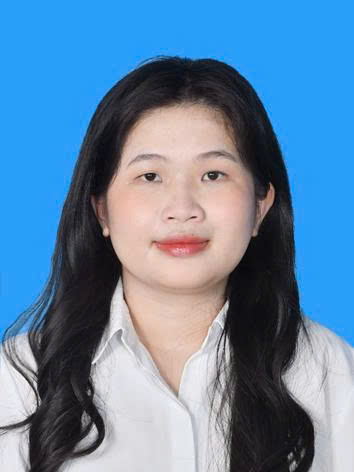
\includegraphics[
        width=2.1cm,
        height=2.5cm,
        keepaspectratio
    ]{assets/avt.jpg}
\end{minipage}

\end{tabularx}

\vspace{2pt}
\textcolor{rulecol}{\rule{\linewidth}{0.6pt}}

% ─── MỤC TIÊU ─────────────────────────────────────────

\section*{Mục tiêu nghề nghiệp}

{\small
Sinh viên năm cuối ngành Công nghệ Thông tin định hướng AI Engineer,
có kinh nghiệm thực hành về Computer Vision, Deep Learning và Python.
Đã phát triển, huấn luyện và tích hợp các mô hình YOLO, CNN, Siamese
Network, MediaPipe và Transformer. Mong muốn phát triển các giải pháp
AI thực tế và nâng cao chuyên môn về AI Model Development \& Deployment.
}

% ─── HỌC VẤN ──────────────────────────────────────────

\section*{Học vấn}

\entry
{Trường Đại học Giao thông Vận tải TP. Hồ Chí Minh (UTH)}
{10/2022 -- 10/2026}
{Cử nhân Công nghệ Thông tin -- Đã hoàn thành chương trình học}

{\small
\begin{cvitems}
    \item GPA: \textbf{3.4 / 4.0}
    \item \textbf{Học bổng Khuyến khích học tập loại Xuất sắc} -- Học kỳ 1, 2025
    \item \textbf{Giải Nhì -- Bảng AI}, Hội nghị Sinh viên Nghiên cứu Khoa học UTH 2025
\end{cvitems}
}

% ─── KỸ NĂNG ──────────────────────────────────────────

\section*{Kỹ năng chuyên môn}

{\small
\begin{tabularx}{\linewidth}{@{}lX@{}}

\textbf{AI / ML}
&
Machine Learning, Deep Learning, Computer Vision, CNN,
YOLO, Siamese Network, Transformer
\\[1pt]

\textbf{Computer Vision}
&
Object Detection, Pose Estimation, Image Classification,
Face Recognition, Image Processing, MediaPipe
\\[1pt]

\textbf{AI Development}
&
Python, PyTorch, OpenCV, Ultralytics YOLO, NumPy, Pandas, FastAPI
\\[1pt]

\textbf{Models}
&
YOLOv8, YOLO Pose, CNN, Siamese Network, Transformer Encoder,
ArcFace, MediaPipe
\\[1pt]

\textbf{Backend / Data}
&
FastAPI, RESTful API, PostgreSQL, SQL Server, MongoDB,
Firebase, Supabase
\\[1pt]

\textbf{Tools}
&
Git, Docker, Postman, VS Code, Power BI, Airflow, dbt

\end{tabularx}
}

% ─── KINH NGHIỆM ──────────────────────────────────────

\section*{Kinh nghiệm làm việc}

\entry
{Gotik Consulting -- Data Engineer}
{Python \textbar{} dbt \textbar{} PostgreSQL \textbar{} Airflow}
{03/2026 -- 05/2026}

{\small
\begin{cvitems}
    \item Xử lý và biến đổi dữ liệu Odoo phục vụ phân tích và báo cáo.
    \item Xây dựng pipeline dữ liệu bằng Python, dbt và Neon PostgreSQL.
    \item Tự động hóa quy trình xử lý dữ liệu theo giờ bằng Apache Airflow.
\end{cvitems}
}

% ─── DỰ ÁN ────────────────────────────────────────────

\section*{Dự án AI tiêu biểu}

\entry
{Fall Detection -- Hệ thống phát hiện té ngã thời gian thực}
{Python \textbar{} YOLOv8 Pose \textbar{} MediaPipe \textbar{} Transformer \textbar{} FastAPI}
{04/2026 -- 06/2026}

{\small
\begin{cvitems}
    \item Phát triển hệ thống Computer Vision phát hiện té ngã sử dụng YOLOv8 Pose, MediaPipe và Transformer.
    \item Huấn luyện Transformer Encoder với đầu vào 30-frame $\times$ 200-feature để phân loại té ngã/không té ngã.
    \item Đạt \textbf{97.8\% mean accuracy} với 5-fold cross-validation và tích hợp FastAPI.
    \item GitHub: \href{https://github.com/hohuynhnhu/Fall-Detection}{Fall-Detection}
\end{cvitems}
}

\vspace{2pt}

\entry
{VehicleScan -- Hệ thống bãi đỗ xe thông minh AI \& IoT}
{Python \textbar{} YOLO \textbar{} CNN \textbar{} Siamese Network \textbar{} ESP32}
{03/2025 -- 03/2026}

{\small
\begin{cvitems}
    \item Phát triển mô hình phát hiện và nhận diện phương tiện sử dụng YOLO, CNN và Siamese Network.
    \item Chuẩn bị dataset và huấn luyện mô hình AI phục vụ nhận diện phương tiện thời gian thực.
    \item Tích hợp AI với ESP32 và Firebase; đạt \textbf{Giải Nhì -- Bảng AI} tại UTH 2025.
    \item GitHub: \href{https://github.com/LeKhang-cn22h/VehicleScanner.git}{VehicleScanner}
\end{cvitems}
}

% ─── THÔNG TIN BỔ SUNG ────────────────────────────────

\section*{Thông tin bổ sung}

{\small
\begin{tabularx}{\linewidth}{@{}lX@{}}

\textbf{Kỹ năng mềm}
&
Giải quyết vấn đề \textbar{} Tự học và nghiên cứu \textbar{}
Làm việc nhóm \textbar{} Khắc phục sự cố
\\[1pt]

\textbf{Tiếng Anh}
&
Đọc hiểu tài liệu kỹ thuật và giao tiếp cơ bản trong công việc
\\[1pt]

\textbf{Thời gian làm việc}
&
Sẵn sàng làm việc toàn thời gian và thích nghi với yêu cầu công việc.

\end{tabularx}
}

\end{document}

